% !TEX root = main.tex

\section{Trading Graph Construction}
Using effective graph analytics, we can investigate more information hidden behind transaction data on blockchain. For example, by analyzing the Ethereum trading graph (ETG, for short), we can classify accounts as different identities which are introduced before. In this section, we first introduce the definition of the basic concepts in trading graph embedding, and then construct multi-layer trading graph.

\subsection{Notation and Problem Definition}
Intuitively, we consider the ETG as $G=(V,E)$, where $v \in V$ is a node and $e \in E$ is an edge. Actually node $v$ represent an address in Ethereum and $V$ is the set of addresses in which includes both EOAs and SCs. We use the terms address and node interchangeably in the remainder of this paper. $E$ is a set of ordered pairs, where $E=\{(v_i,v_j)|v_i,v_j \in V\}$. The order of an edge indicates the direction of activity (e.g., assets transfer and smart contract invocation) from $v_i$ to $v_j$. 
%In our definition, each edge associates with a weight $w$, which will be discussed later. Hence, $G$ is a weighted directed graph.

We define our problem as follows: Given ETG $G=(V,E)$, we aim to represent each node $v$ in a low-dimensional vector space $\vec{y_v}$. By representing ETG as a set of low dimensional vectors, graph algorithms can then be computed efficiently. Generally network embedding techniques such as random-walk based and deep learning based models use the pure network structure to map into the embedding space\cite{goyal2018capturing}. However, ETG is different from traditional network such as social media networks and citation graph, specific challenges as follows. 

\begin{itemize}
\item Edges in ETG include multiple activities such as assets transfer and smart contract invocation, which are radically different from one another and can not be measured in a uniform weight model.
\item In ETG, two nodes are more similar if they have similar neighborhood structures instead of they are just connected by an edge with larger weight simply. Using node adjacency as the input, most graph embedding techniques can not preserve such higher order proximity.
\end{itemize}

\subsection{ETG Division}

\begin{figure}[htbp]
	\centering
	\label{fig}
	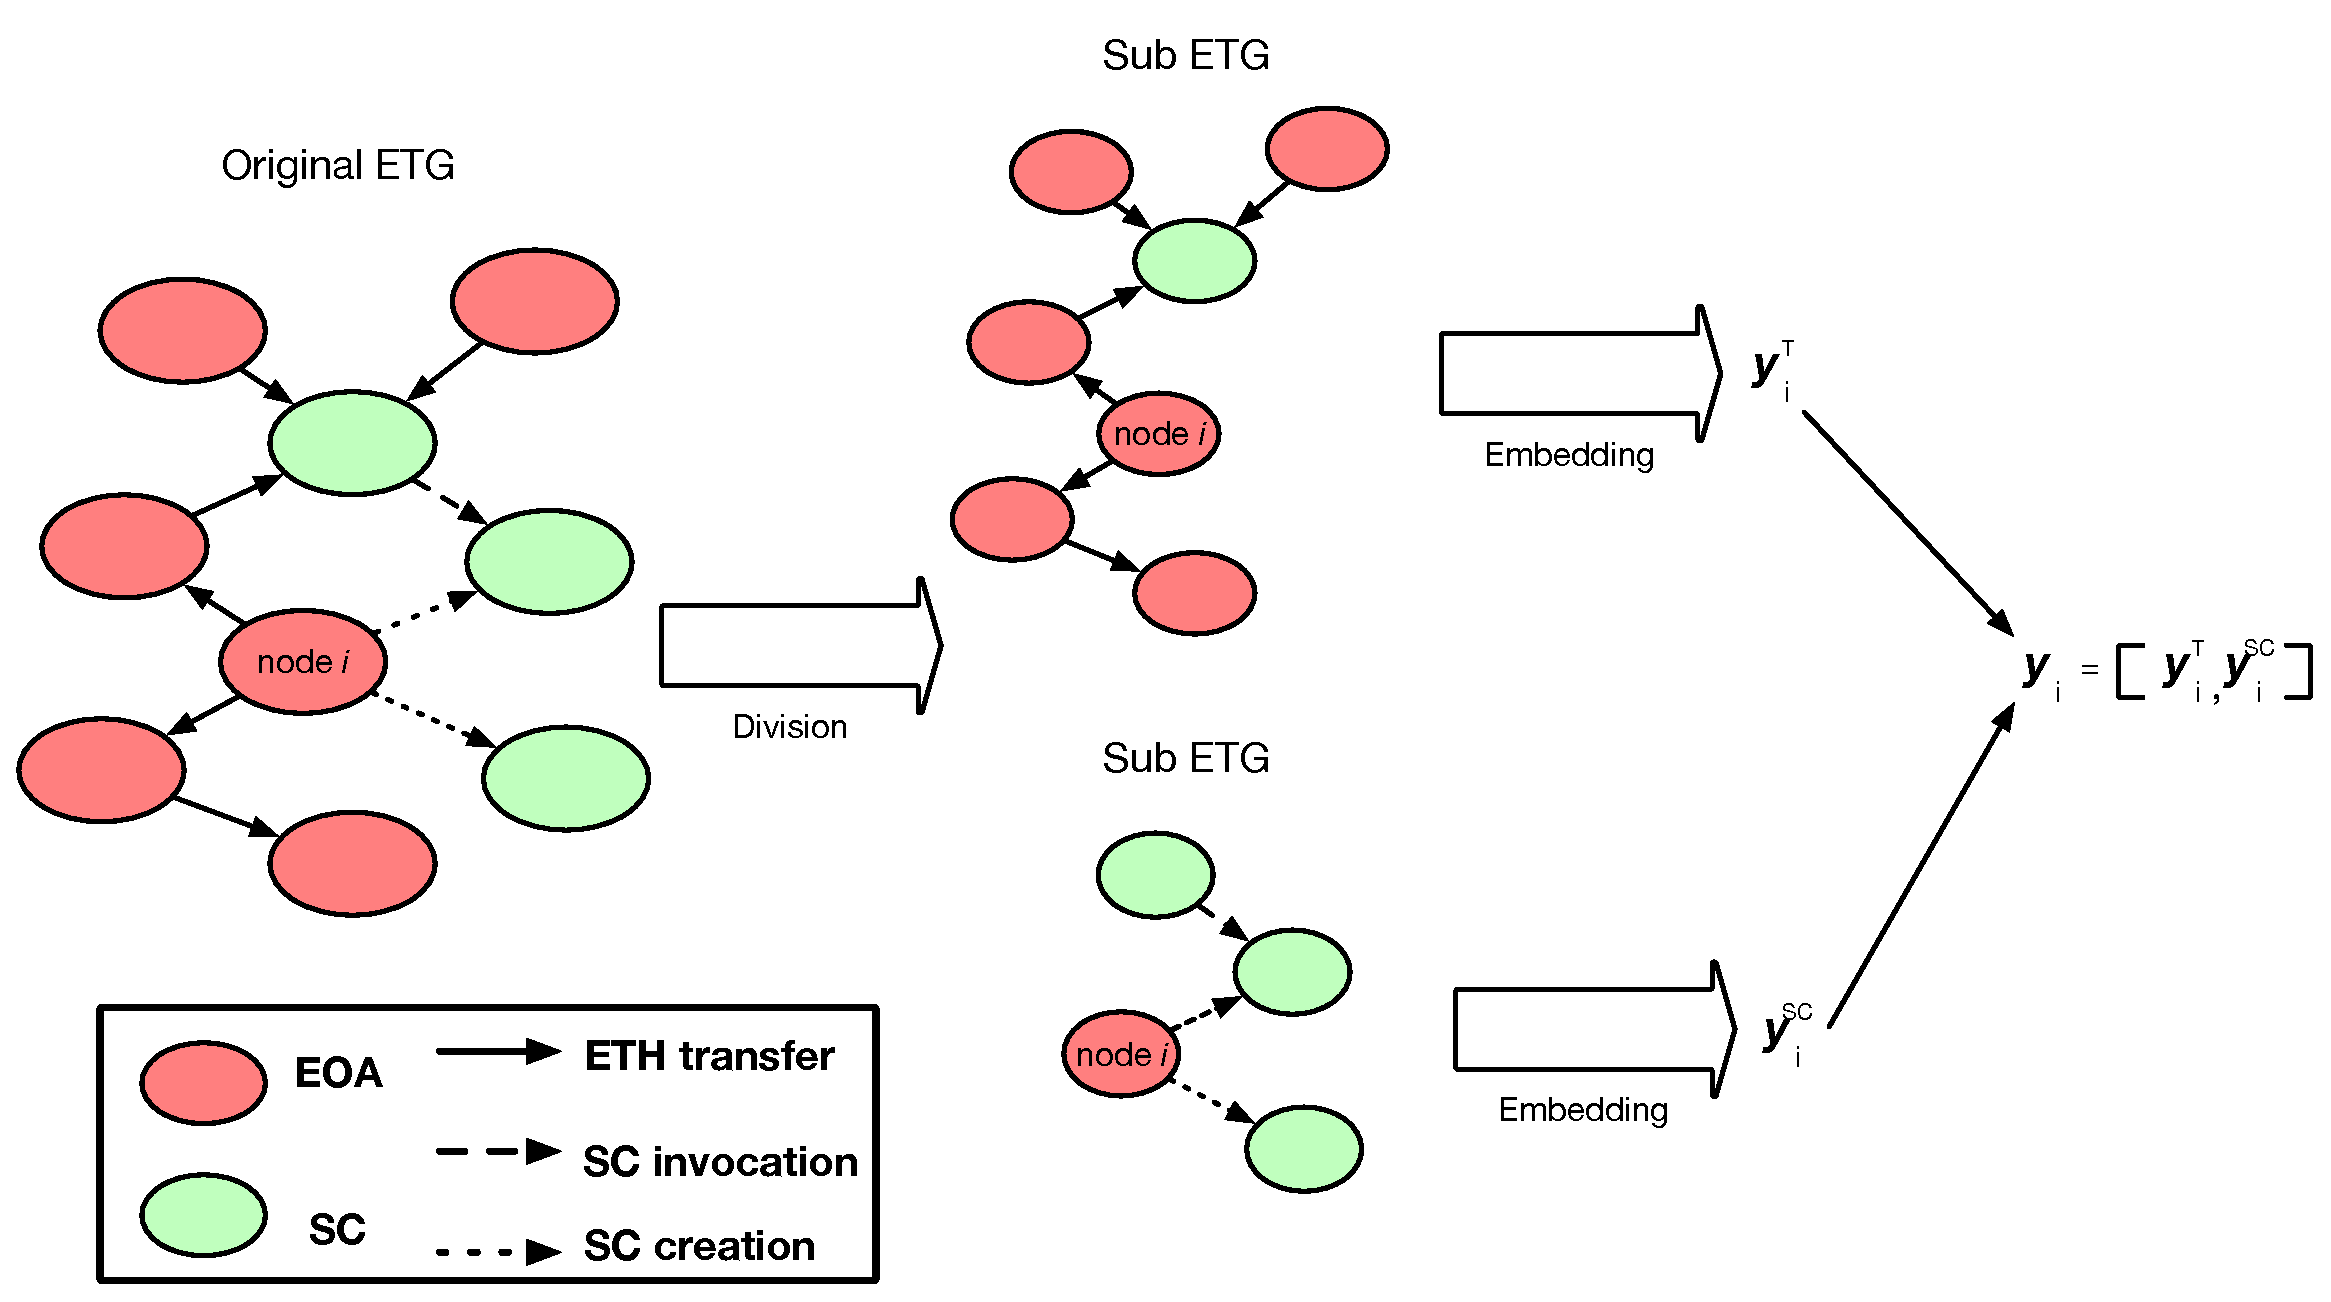
\includegraphics[width=3.5in]{fig/graph_split.eps}
	\caption{Example of a figure caption.}
\end{figure}

Since edges in ETG stand for different activities and can not be measured in a uniform weight model. For example, a weight of assets transfer maybe the ETH amount, however an invocation to smart contract does not have such numerical value. This inspired us to divide the raw ETG into different sub graphs.

\textbf{Definition 1.} $G^{T}=\{V^T,E^T\}$, where $V^T$ is the subset of $V$. $E^T=\{(v_i,v_j,w)|v_i,v_j \in V^T,w \in \mathbb{R^+}\}$ where an edge $(v_i,v_j)$ indicates that there is at least one ETH transfer from node $v_i$ to $v_j$. And $w$ is the summation of all transferred ETH amount from $v_i$ to $v_j$ for a period of time.

Actually, $G^T$ represents the ETH trading activities in Ethereum, and each node in $V^T$ has at least one ETH transaction. Note that ERC-20 transactions are not accounted for in the graph because the transaction value is $0$ in an ERC-20 \emph{CALL} transaction. Another reason is that even converting some ERC-20 tokens into ETH is available, the exchange-rate fluctuations make the unification meaningless.

\textbf{Definition 2.} $G^{SC}=\{V^{SC},E^{SC}\}$, where $V^{SC}$ is the subset of $V$. $E^{SC}=\{(v_i,v_j,w)|v_i,v_j \in V^{SC},w \in \mathbb{R^+}\}$ where an edge $(v_i,v_j)$ indicates that there is at least one smart contract creation or invocation from node $v_i$ to $v_j$. It is easy to find out that all SC address 

%And $w$ is the summation of all transferred ETH amount from $v_i$ to $v_j$ for a period of time.